\RequirePackage{luatex85}
\documentclass{standalone}
\usepackage{tikz}
\usetikzlibrary{decorations}
\usetikzlibrary{decorations.pathmorphing}
\usetikzlibrary{arrows.meta}
\tikzset{>=latex, line width=1.0pt}
\usepackage{amsmath}
\usepackage{mathtools}
\newcommand{\ct}{\hspace{2pt}\rule[1pt]{3pt}{3pt}\hspace{2pt}}
\DeclareMathOperator{\pr}{pr}
\DeclareMathOperator{\transport}{transport}
\usetikzlibrary{calc}
\begin{document}
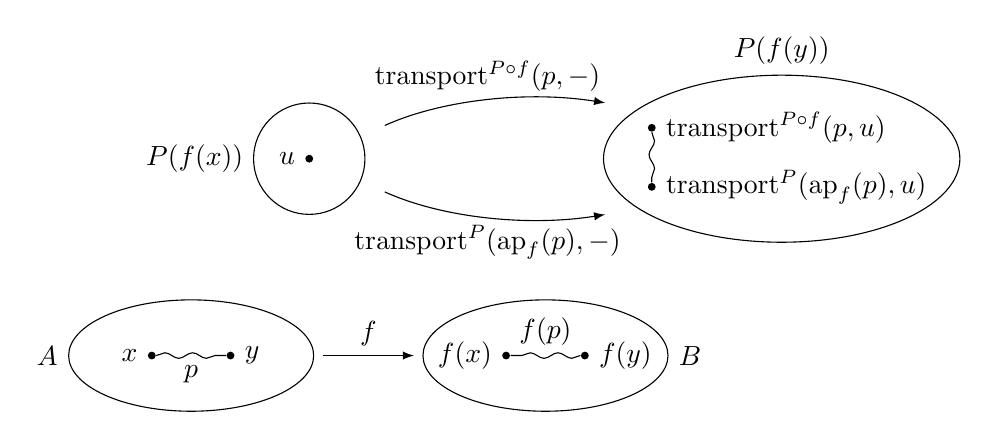
\begin{tikzpicture}[yscale=.5,xscale=1]
  \def\xshift{3}
  \def\yheight{5}

  % P(x)
  \node[circle,draw,inner sep=0.5cm,label=left:{$P(f(x))$}] (px) at (-1.0*\xshift,\yheight) {};
  \node[circle,fill,inner sep=1pt,label=left:{$u$}] (u) at (px) {};

  % P(y)
  \node[circle,draw,inner sep=0.5cm,label=above:{$P(f(y))$},yscale=1.5,xscale=3.2] (py) at (1.0*\xshift,\yheight) {};
  \node[circle,fill,inner sep=1pt,label=right:{$\mathrm{transport}^{P\circ f}(p,u)$},yshift=0.5] (tpfu) at (0.45*\xshift,1.15*\yheight) {};
  \node[circle,fill,inner sep=1pt,label=right:{$\mathrm{transport}^{P}(\mathrm{ap}_f(p),u)$},yshift=0.5] (tpu) at (0.45*\xshift,0.85*\yheight) {};
  \draw[decorate,decoration={snake,amplitude=1}] (tpfu) -- (tpu);

  % P(x) -> P(y)
  \draw[->,shorten >=0.3cm,shorten <=0.3cm, transform canvas={yshift=0.1cm}] (px) to[bend left] node[above] {$\mathrm{transport}^{P\circ f}(p,-)$} (py) {};
  \draw[->,shorten >=0.3cm,shorten <=0.3cm, transform canvas={yshift=-0.1cm}] (px) to[bend right] node[below] {$\mathrm{transport}^{P}(\mathrm{ap}_f(p),-)$} (py) {};

  % Base space B
  \node[circle,draw,inner sep=0.5cm,label=right:{$B$},xscale=2.2] (B) at (0,0) {};
  \node[circle,fill,inner sep=1pt,label=left:{$f(x)$}] (fy) at (-.5,0) {};
  \node[circle,fill,inner sep=1pt,label=right:{$f(y)$}] (fx) at (.5,0) {};
  \draw[decorate,decoration={snake,amplitude=1}] (fx) -- node[auto,swap] {$f(p)$} (fy);

  % Base space A
  \node[circle,draw,inner sep=0.5cm,label=left:{$A$},xscale=2.2] (A) at (-1.5*\xshift,0) {};
  \node[circle,fill,inner sep=1pt,label=left:{$x$}] (b1) at (-.5-1.5*\xshift,0) {};
  \node[circle,fill,inner sep=1pt,label=right:{$y$}] (b2) at (.5-1.5*\xshift,0) {};
  \draw[decorate,decoration={snake,amplitude=1}] (b1) -- node[auto,swap] {$p$} (b2);

  \draw[->,shorten >=0.1cm,shorten <=0.1cm] (A) to[] node[auto] {$f$} (B) {};

  % \draw[->] (-0.5*\xshift,\yheight+0.2*\yheight) to[bend left] node[auto] {$p_\ast$} (0.5*\xshift,\yheight+0.2*\yheight);
\end{tikzpicture}
\end{document}